% Begin Netzwerk Design
\section{Netzwerk Klassendiagramm}

\begin{figure}[H]
  \begin{center}
		\rotatebox{90}{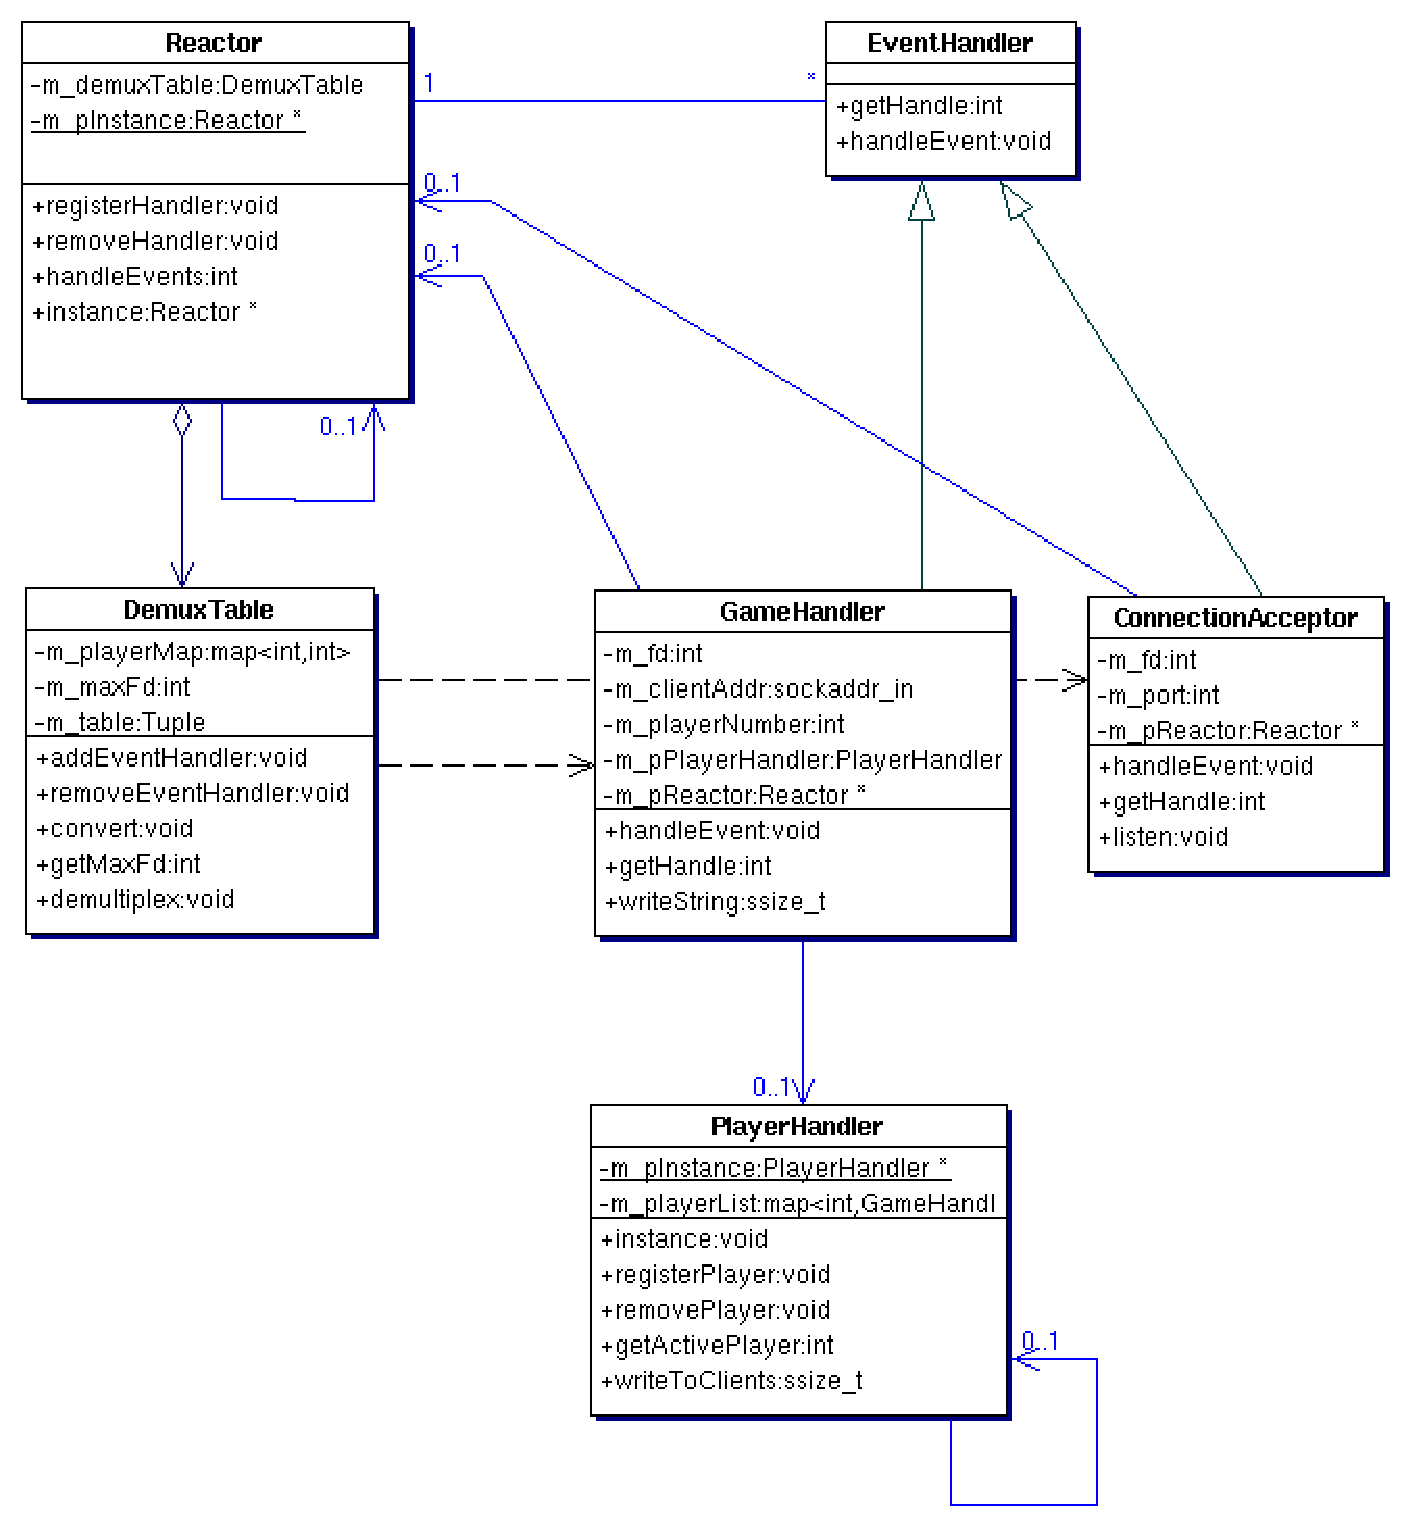
\includegraphics[width=12cm]{./images/reactor_klassendiagramm.pdf}}
  \end{center}
  \caption{Klassendiagramm Netzwerk/Server}
\end{figure}

\subsection{Beschreibung des Reactor Patterns}
Das Problem, dass sich bei einem Spiel, das erstens gewissen Geschwindigkeitsanforderungen gen"ugen muss und zweitens mehrere 
(mehr als 2) Mitspieler hat, ist, dass die Netzerwerkkommunikation speziell gel"ost werden muss, da alle Clients zu einem
nicht vorhersehbaren Zeitpunkt Meldungen zum Server schicken k"onnen. Da die Systemfunktionen, die f"ur die Kommunikation ben"otigt
werden (also read() und write() ) blockierend sind, muss entweder f"ur jeden Client ein seperater Prozess gestartet werden oder es 
muss ein geeignetes Pattern verwendet werden. Die erste L"osung w"are sehr einfach zu implementieren (wird auch sehr oft gemacht, zum
Beispiel bei Web Anwendungen), hat aber den Nachteil, dass bei einer Anwendung wie der unsrigen Interprozesskommunikation erforderlich
gewesen w"are, was sehr m"uhsam zu implementieren ist und auch Performance Nachteile mit sich bringt.
Die zweite L"osung mit dem Pattern erschien uns deshalb vorteilhafter, obwohl es auch nicht einfacher zu implementieren ist, 
aber die sinnvollere L"osung f"ur ein Spiel ist. 

Das Reactor Pattern hat folgende Vorteile
\begin{itemize}
	\item Wartezeiten und Antwortezeiten des Servers werden k"urzer da nicht blockierend auf einen Event eines einzigen Clients gewartet wird.
	\item Datendurchsatz wird erh"ort, da keine Daten zwischen einzelnen Prozessen ausgetauscht werden m"ussen.
	\item Sehr gute Wartungs- und Erweiterungseigenschaften, da "Anderungen nur an einem Ort gemacht werden m"ussen.
	\item Es ist kein Multithreading und keine Synchronisation im Server n"otig
\end{itemize}

Erreicht wird dies, indem synchron auf das Eintreffen von Ereignissen von verschiedenen Orten (Clients) gewartet wird. Diese Ereignisse
werden entgegengenommen, ausgewertet und an die bereitgestellten services weitergeleitet. Die Klassen und Methoden des Reactor 
Patterns werden in den folgenden Abschnitten erkl"art.
	
	
\subsection{Klasse Reactor (Singleton)}
Die Klasse ist daf"ur verantwortlich, die select() Funktion aufzurufen und anhand der Resultate, die sie von dieser Funktion erh"alt,
Reaktionen auszuf"uhren. Das heisst konkret, dass die select() Funktion, welche eine System Funktion ist, eine Meldung gibt, wenn ein 
Event eintrifft. Falls dies geschieht, ist die Reactor Klasse daf"ur verantwortlich, das richtige Handler Objekt (ConnectionAcceptor oder
GameHandler) aufzurufen. Damit stellt diese Klasse eine Abstraktion der select() Funktion dar und ist daf"ur verantwortlich, dass die
Handler Funktionen read() und connect() nur aufgerufen werden, wenn es tats"achlich n"otig ist. Damit wird gew"ahrleistet, dass
das System nicht blockiert, sondern dass alle Clients sehr schnell bedient und abgefragt werden k"onnen.
\subsubsection{Funktionen}
\begin{tabular}{p{50mm}p{90mm}}
	+registerHandler(EventHandler* pEventHandler, EventType eventType) : void  &  registriert einen neuen Event Handler (ConnectionAcceptor
	oder GameHandler) mit dem dazugeh"origen Event Typ in der Demultiplex Tabelle. \\
	+removeHandler(EventHandler* pEventHandler, EventType eventType)  : void  &  entfernt den Event Handler aus der Demultiplex Tabelle \\
	+handleEvents() : int     & f"uhrt die select() Funktion aus und ruft die 
	entsprechende Methode im ConnectionAcceptor bzw. im GameHandler auf. \\
	+instance() : Reactor* & gibt die Reactorinstanz zur"uck. \\ 
\end{tabular}


\subsection{Klasse EventHandler}
Diese Klasse ist eine rein virtuelle Klasse und stellt die Schnittstelle f"ur die abgeleiteten Klassen ConnectionAcceptor und GameHandler dar.

\subsection{Klasse ConnectionAcceptor}
Der ConnectionAcceptor ist daf"ur zust"andig, Verbindungsanfragen zu regeln. Das heisst, wenn sich ein Client mit dem Server verbinden m"ochte,
macht der ConnectionAcceptor eine neue Verbindung auf der Serverseite (erstellt einen neuen Filedeskriptor)
und falls es keine Fehler dabei gibt, wird ein neuer GameHandler erstellt.
\subsubsection{Funktionen}
\begin{tabular}{p{50mm}p{90mm}}
	+listen() : void & stellt einen Filedeskriptor mit der richtigen Struktur um Verbindungsanfragen entgegenzunehmen zur Verf"ugung und 
	registriert diesen beim Reactor. \\
	+handleEvent(int fd, EventType eventType) : void & ist eine "uberschriebene Funktion der Klasse EventHandler. Diese ist zust"andig, ankommende
	Anfragen f"ur eine Verbindung entgegenzunehmen und wenn kein Fehler auftritt, wird die Verbindung akzeptiert und ein neues GameHandler Objekt erstellt. \\
	+getHandle() : int & gibt den Filedeskriptor, der in der listen() Funktion bereitgestellt wurde zur"uck. \\
\end{tabular}

\subsection{Klasse GameHandler}
F"ur jeden Client, der sich verbunden hat, gibt es ein GameHandler Objekt. Dieses Objekt regelt die ganze Kommunikation zwischen Client und
Server f"ur diesen bestimmten Client. Das heisst, er nimmt alles, was vom Client zum Server geschickt wird entgegen und schreibt alles
vom Server zum Client. 
\subsubsection{Funktionen}
\begin{tabular}{p{50mm}p{90mm}}
	+handleEvent(int fd, EventType eventType) : void & ist eine "uberschriebene Funktion der Klasse EventHandler. Sie nimmt die
	Strings, die vom Client an den Server "ubermittelt wurden an und gibt diese an die PD weiter. \\
	+getHandle() : int & gibt den Filedeskriptor, der den GameHandler identifiziert zur"uck. \\
	+writeToClient(const char* str, size\_t n) : ssize\_t & Schreibt die Strings, die von der PD an die Clients "ubermittelt werden sollen zu dem
	Client, f"ur den das GameHandler Objekt zust"andig ist. \\
\end{tabular}

\subsection{Klasse DemuxTable}
Die Demultiplex Tabelle ist dazu da, die Filedeskriptoren mit ihren entsprechenden Eventtypen zu registrieren, 
damit bei einer Anfrage des Clients das richtige GameHandler Objekt
aufgerufen werden kann. Das heisst in dieser Tabelle sind alle File Deskriptoren mit den zugeh"origen Events gespeichert.
\subsubsection{Funktionen}
\begin{tabular}{p{50mm}p{90mm}}
	+convert(fd\_set\& read\_fds, fd\_set\& except\_fds) : void & konvertiert die Event-Typen um herauszufinden, was f"ur ein Event ansteht 
	(ein read oder connect Event)\\
	+addEventHandler(int fd, EventHandler* pEventHandler, EventType eventType) : void & ein EventHandler wird mit seinem Event Typ 
	in der Tabelle registriert.\\
	+removeEventHandler(int fd) : void & der EventHandler wird wieder aus der Tabelle entfernt.\\
	+getMaxFd() : int & der Zahlenwert des gr"ossten Filedeskriptors wird zur"uckgegeben.\\
	+demultiplex(int fdCount, fd\_set\& read\_fds, fd\_set\& except\_fds) : void & es wird anhand des Event-Typs in der Tabelle
	und des anstehenden Events herausgefunden, welche handleEvent() Funktion aufgerufen werden muss.\\
\end{tabular}

\section{Klasse PlayerHandler(Singleton)}
Im Netzwerk werden noch Assoziationen zwischen Filedeskriptor und Player (also Client) gemacht. Die PlayerHandler Klasse ist
von der Funktion her (nicht vom Aufbau) "ahnlich wie die Demultiplex Tabelle. Sie speichert f"ur jeden Client, also f"ur jeden GameHandler
einen Zeiger, damit sie diesen kennt. Wenn nun eine Meldung von der ServerPD an die Clients geschickt werden soll, wird in dieser Klasse
die entsprechende write() Funktion in allen GameHandler Objekten aufgerufen.
\subsubsection{Funktionen}
\begin{tabular}{p{50mm}p{90mm}}
	+registerPlayer(GameHandler* pGameHandler) : void & Wenn sich ein neuer Spieler angemeldet hat, wird hier das zugeh"orige GameHandler
	Objekt, das den Spieler identifiziert, registriert\\
	+removePlayer(GameHandler* pGameHandler) : void & Wenn die Verbindung zu einem Spieler nicht mehr besteht, wird der GameHandler dieses 
	Spielers hier entfernt.\\
	+getActivePlayer(GameHandler* pGameHandler) : int & gibt die Spielernummer (1-4) zur"uck. \\
	+instance() : WriteHandler* & die Instanz des PlayerHandler wird zur"uckgegeben. \\
\end{tabular}


\subsection{Client (Singleton)}
Die Client Klasse steuert die ganze Verbindung auf der Seite des Clients. Er macht die Verbindung zum Server, schickt daten an diesen und liest 
auch die Daten, die vom Server geschickt werden.
\subsubsection{Funktionen}
\begin{tabular}{p{50mm}p{90mm}}
	+makeConnection(const char* strPtr): int & er"offnet eine Verbindung zum Server mit der angegebenen IP\_Nummer und gibt den 
	Filedeskriptor, der diese Verbindung identifiziert zur"uck. \\
	+writeString(const char* str, size\_t n) : ssizt\_t & Schickt eine Meldung zum Server und gibt die L"ange der geschriebenen Zeichenkette
	zur"uck\\
	+readString() : ssize\_t & liest die Meldung vom Server und gibt die L"ange der Nachricht zur"uck. Die Funktion wird in einem
	eigenen Thread ausgef"uhrt, damit eine Meldung m"oglichst schnell entgegengenommen werden kann.\\
	+close() : void & schliesst die Verbindung zum Server \\
	+instance() : WriteHandler* & die Instanz des Clients wird zur"uckgegeben. \\
\end{tabular}


\section{Netzwerk Sequenzdiagramme}

\begin{figure}[H]
  \begin{center}
   \rotatebox{90}{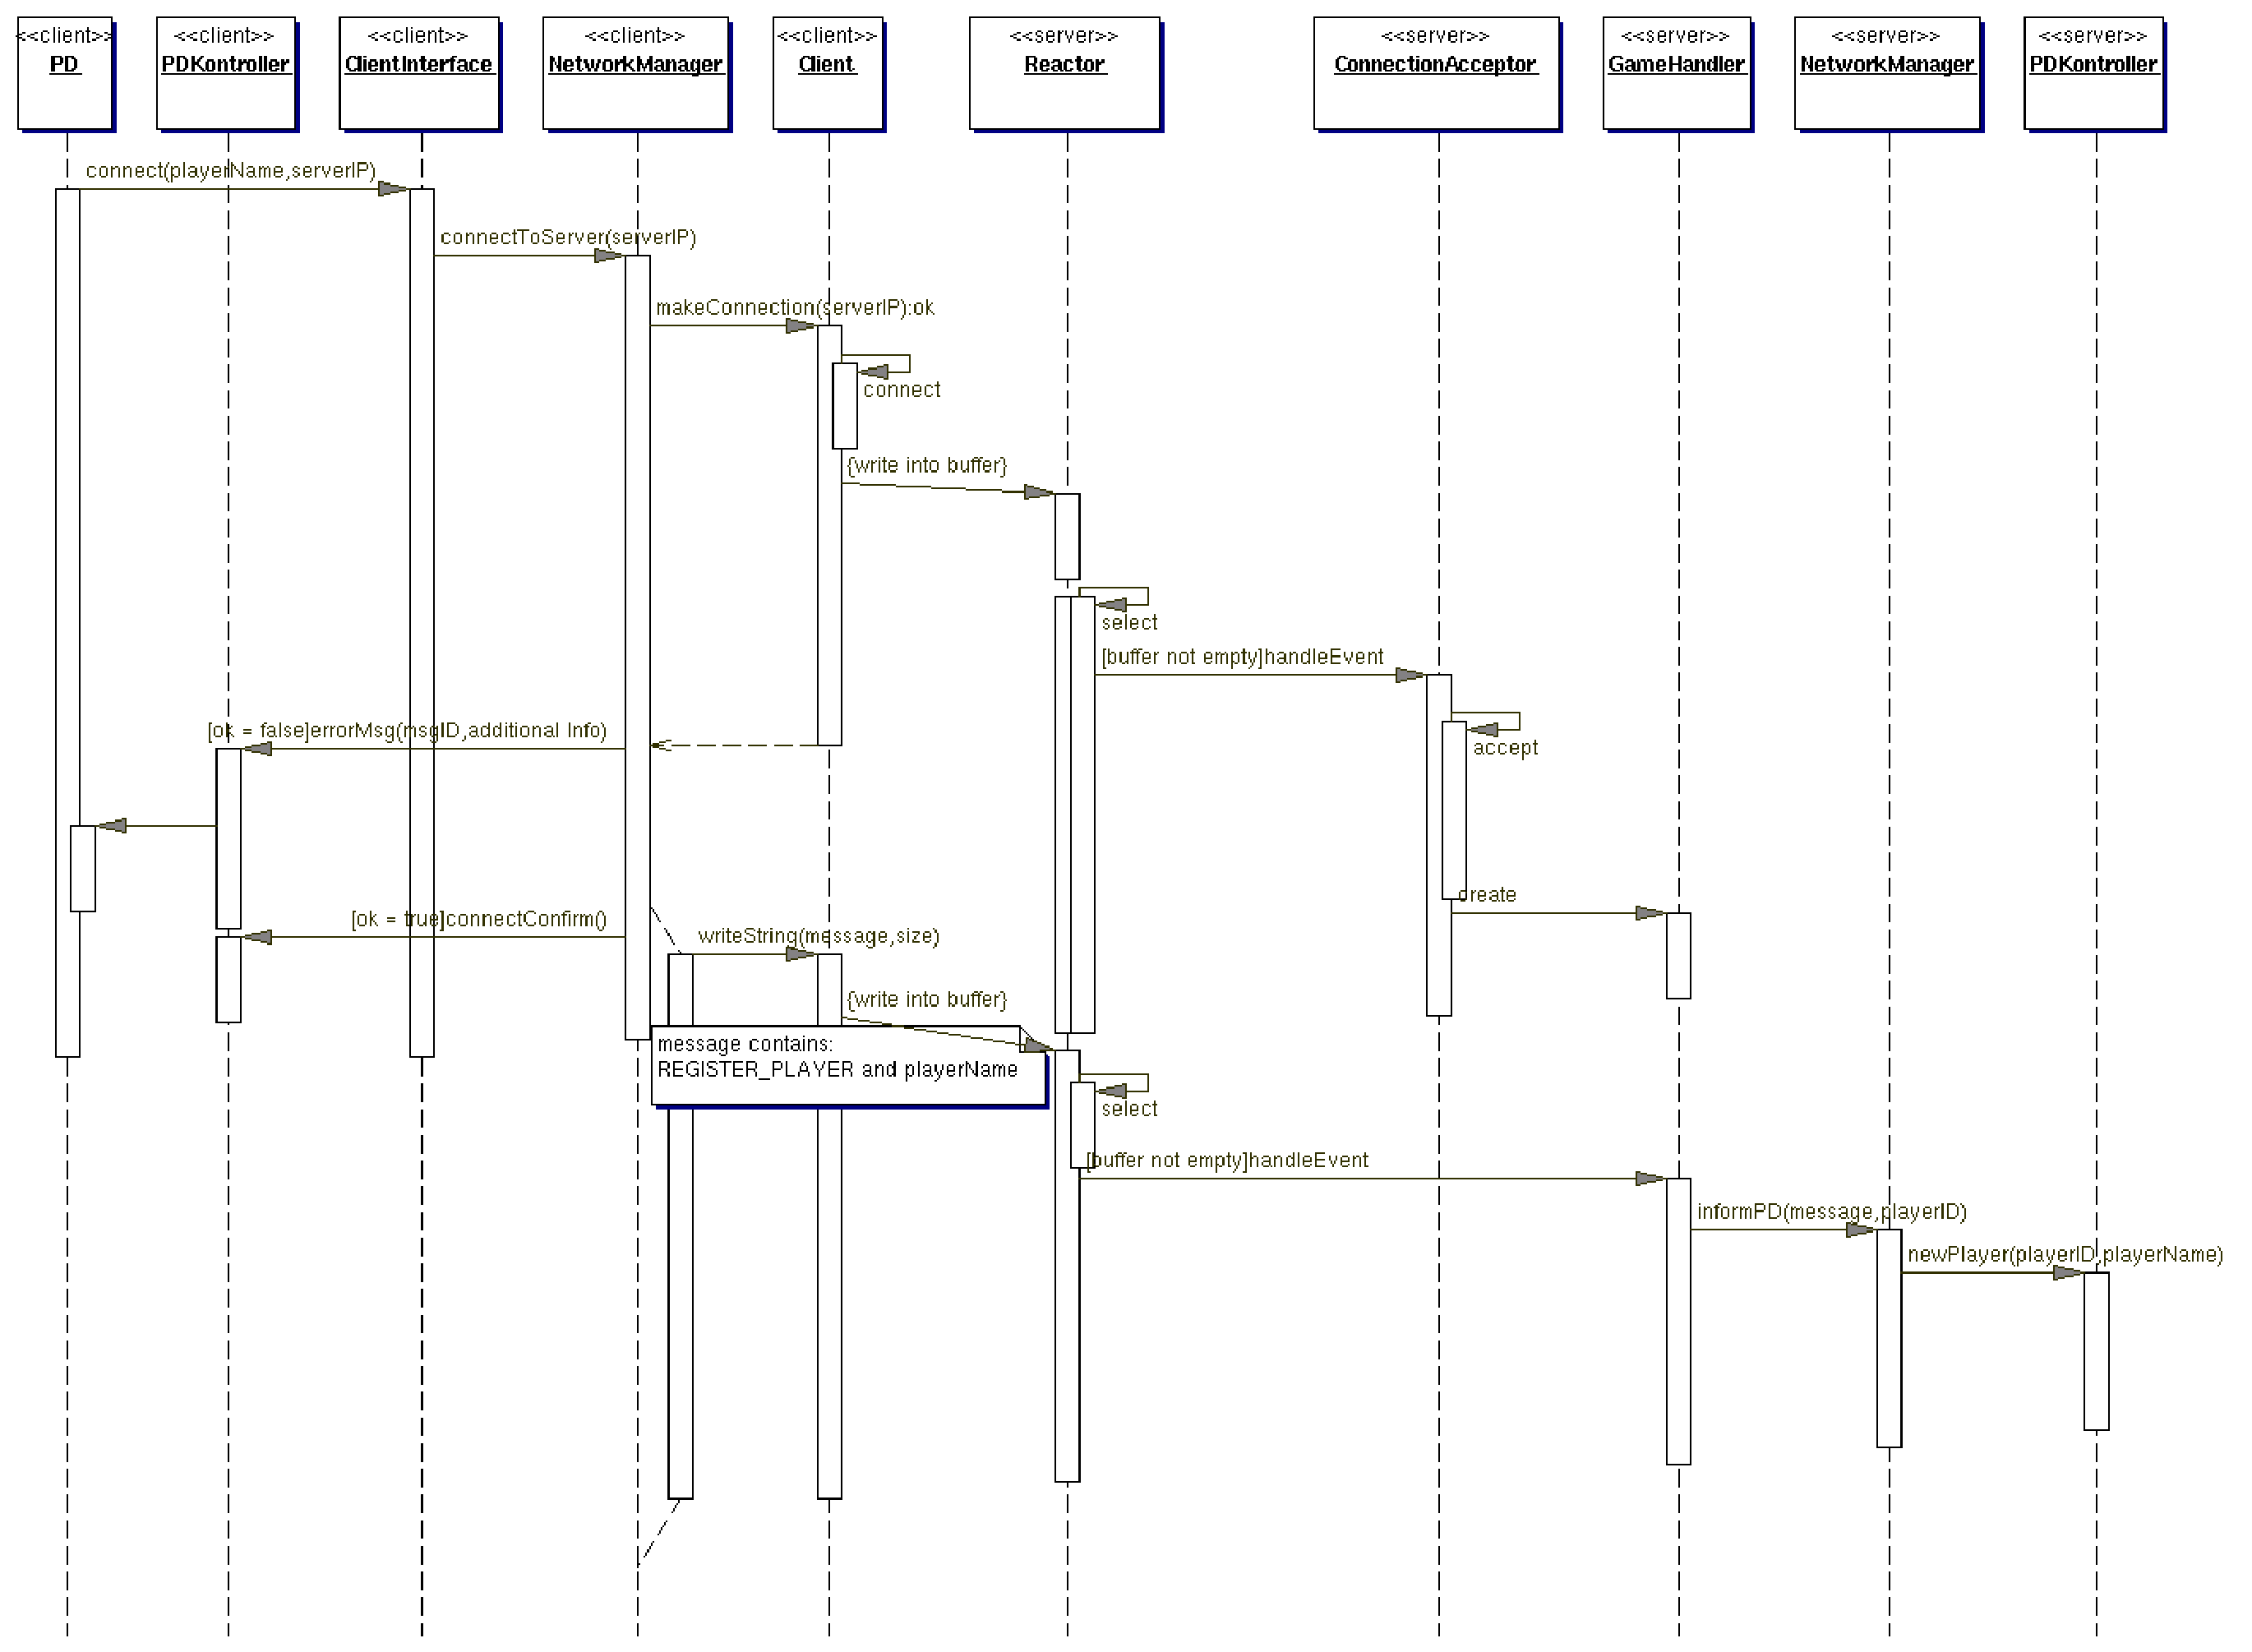
\includegraphics[width=18cm]{./images/clientconnect.pdf}}
  \end{center}
  \caption{Anmeldung des Clients bei einem Spiel}
\end{figure}

\begin{figure}[H]
  \begin{center}
    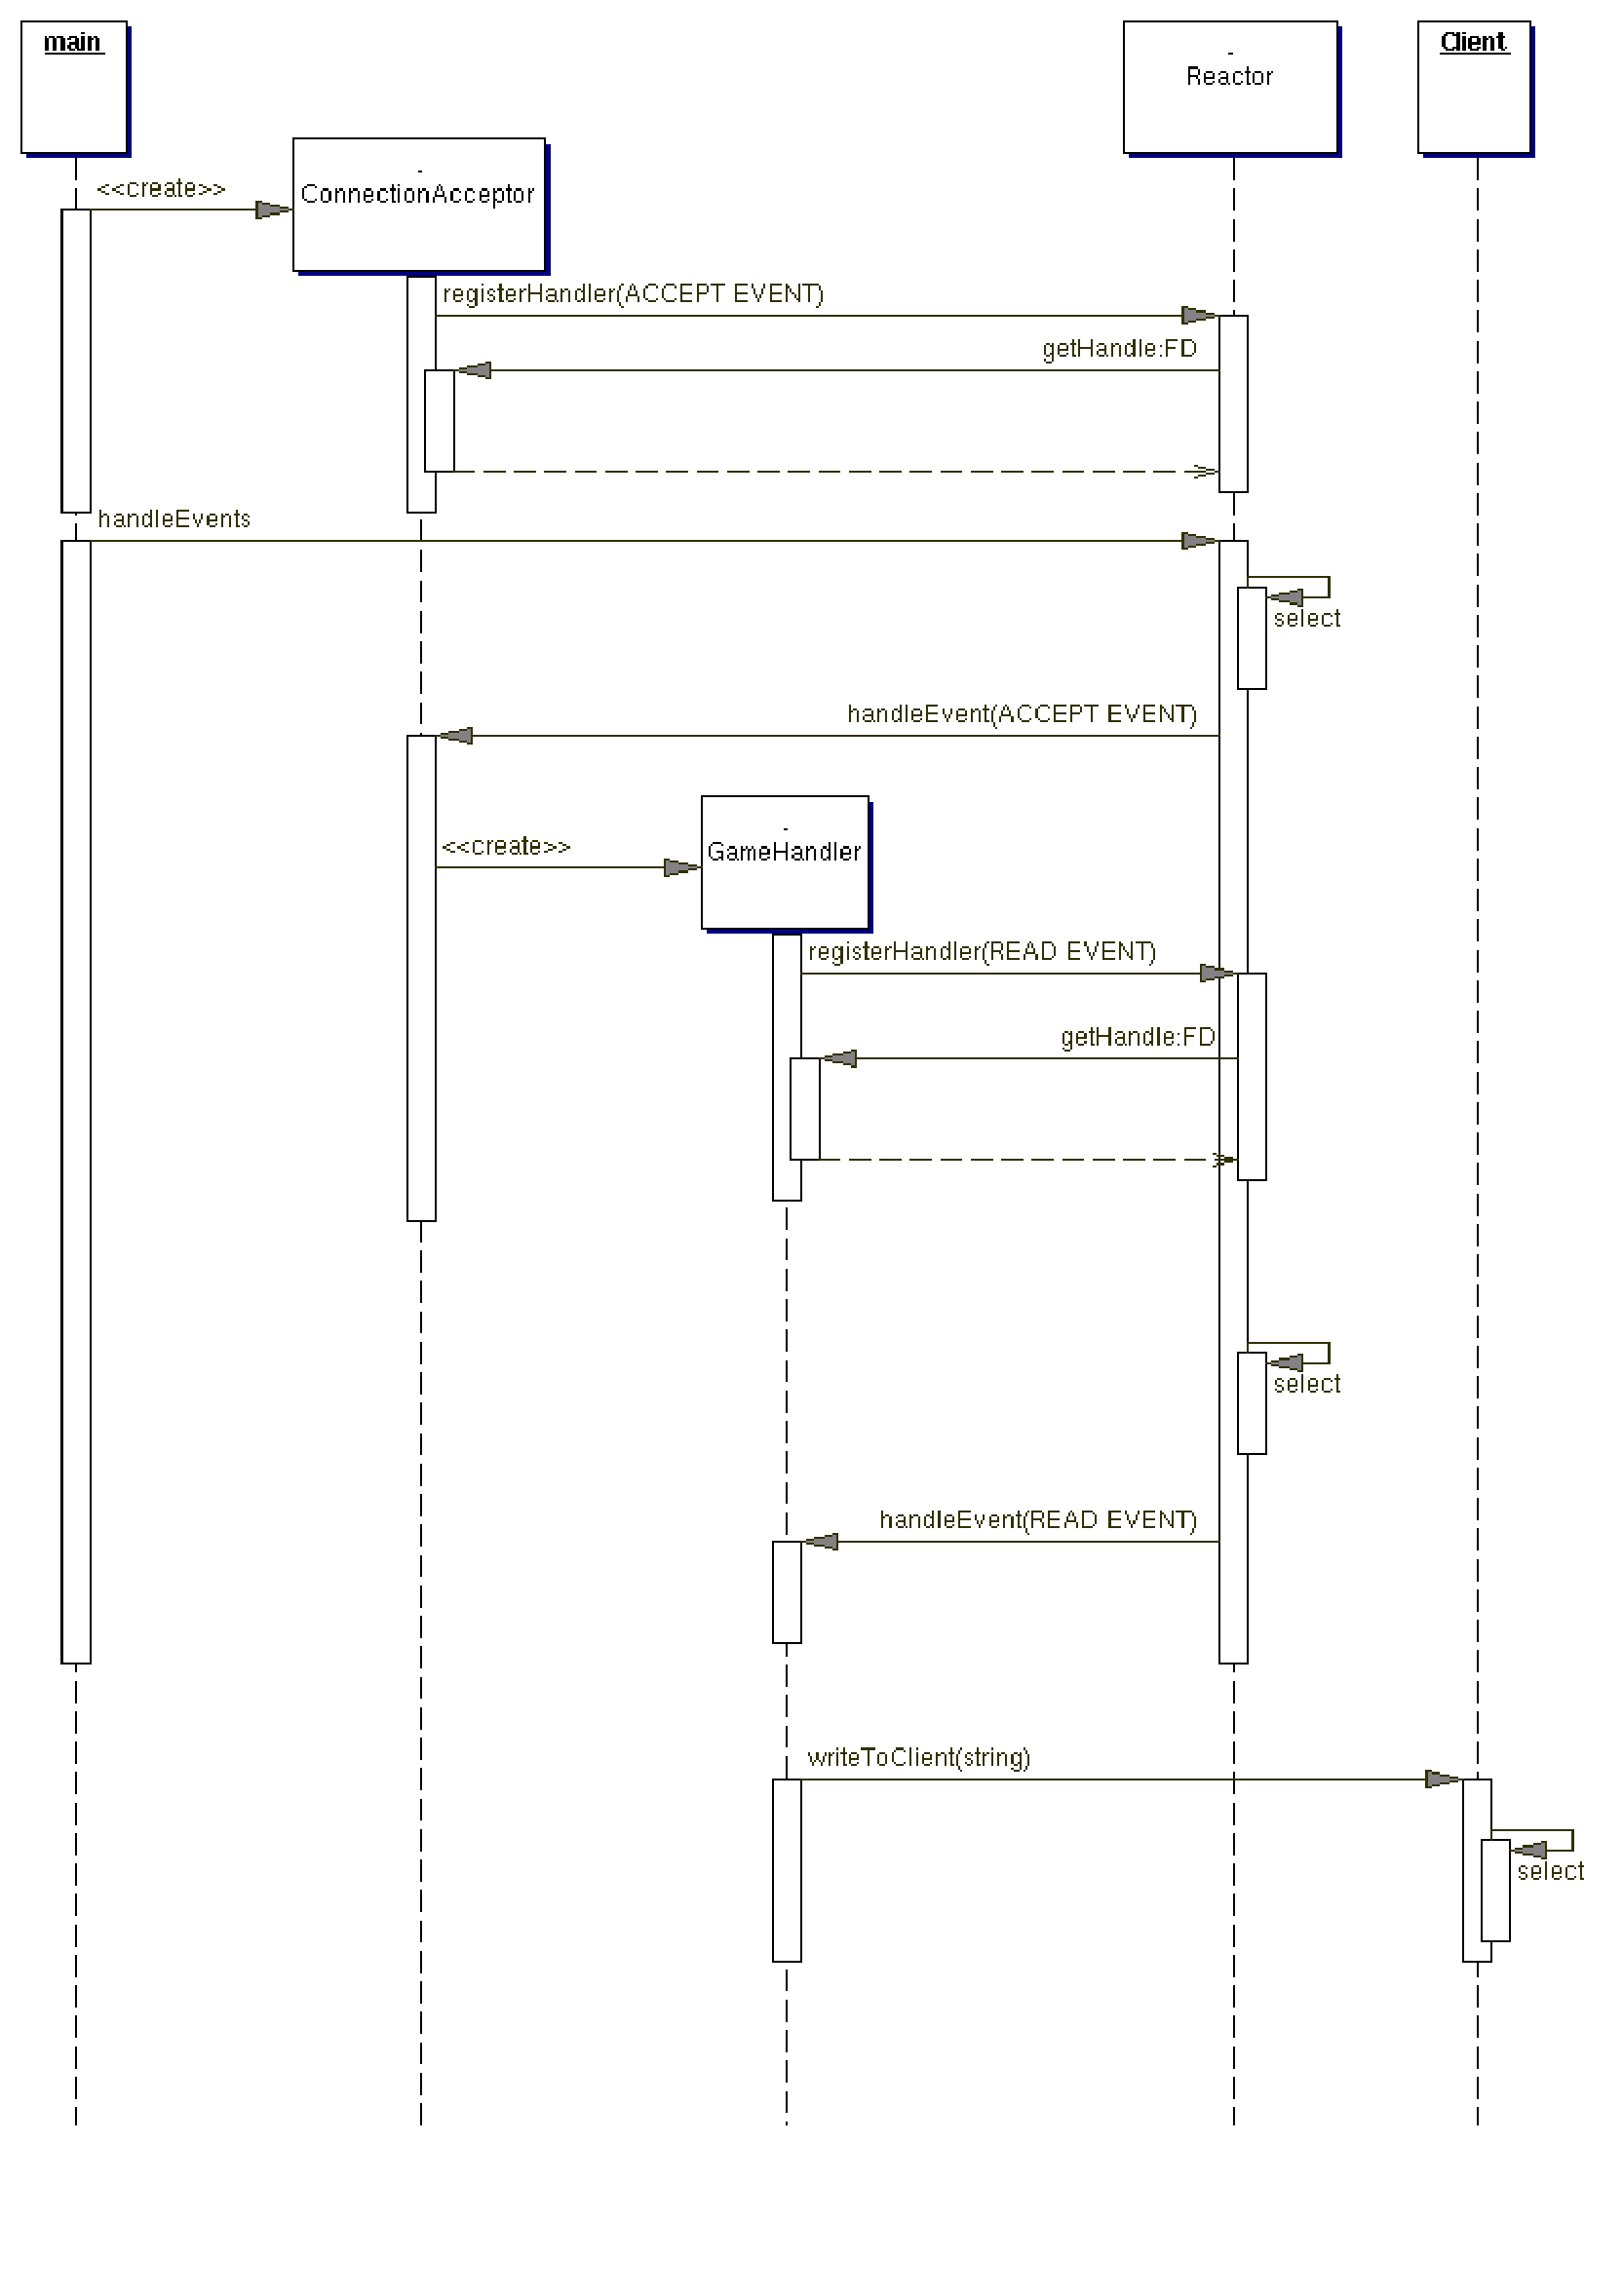
\includegraphics[width=12cm]{./images/sequenz_reactor.pdf}
  \end{center}
  \caption{Sequenzdiagramm Ablauf Server}
\end{figure}

\subsection{Erkl"arung Sequenzdiagramm Ablauf Server}
Im main Programm wird zuerst ein Objekt des ConnectionAcceptor erstellt. Dieser registriert sich anschliessend beim Reactor
und meldet damit, dass er f"ur ACCEPT EVENTS, das heisst f"ur ankommende Anfragen f"ur eine Verbindung, zust"andig ist.
Der Reactor registriert den ConnectionAcceptor in der Demultiplex Tabelle. Damit ist der erste Schritt gemacht und der Server
ist bereit, ankommende Verbindungsanfragen entgegenzunehmen.

Wenn das abgeschlossen ist, wird im Hauptprogramm (in einem eigenen Prozess) fortlaufend die Funktion handleEvents() des 
Reactors aufgerufen. Dieser f"uhrt den Systemaufruf select() durch, der pr"uft, ob eine Anfrage vorhanden ist. Ist dies der 
Fall, pr"uft er die Anfrage und im ersten Schritt wird das eine Verbindungsanfrage sein. Darauf ruft er handleEvent() im ConnectionAcceptor
auf, der die Anfrage entgegennimmt und bearbeitet. Falls es dabei keine Fehler gibt, wird ein neuer GameHandler erzeugt, der sich
gleich wieder beim Reactor registriert, diesmal aber f"ur READ EVENTS. Danach ist der Ablauf derselbe wie im ConnectionAcceptor.

Von nun an wird fortlaufend gepr"uft, ob eine Anfrage anliegt und wenn ja, wird der Typ der Anfrage ermittelt (READ oder ACCEPT Event) 
und die enstprechende Funktion im richtigen Objekt aufgerufen.

%end netzwerk design

